\documentclass[crop=false]{standalone}
% --- ПРЕАМБУЛА ДЛЯ ПОДДЕРЖКИ РУССКОГО ЯЗЫКА И МАТЕМАТИКИ ---
\usepackage[T2A]{fontenc}
\usepackage[utf8]{inputenc}
\usepackage[russian]{babel}
\usepackage{amsmath}
\usepackage{geometry}
\usepackage{amssymb}
\usepackage{graphicx}
\usepackage{float}
\usepackage{import}
\geometry{a4paper, top=2cm, bottom=2cm, left=2cm, right=2cm}
\newcommand{\sidecomment}[1]{\marginpar{\raggedright\scriptsize\itshape #1}}
\newcommand{\iu}{\mathrm{i}}

\newcommand{\Def}{%
    \text{Def}%
    \hspace{-0.85em}% Сдвиг назад ровно на середину (подберите под шрифт)
    \raisebox{0.1ex}{/}% Черта
    \hspace{1em}% Возврат к концу слова + небольшой отступ
}

\renewcommand{\Re}{\operatorname{Re}}
\renewcommand{\Im}{\operatorname{Im}}

\ifstandalone
    \newcommand{\lecturebreak}{} % В отдельном файле лекции разрыв не нужен
\else
    \newcommand{\lecturebreak}{\clearpage} % В полной книге - начинаем с новой страницы
\fi

\newcounter{lecturenumber} % Создаем счетчик для нумерации лекций
\newcommand{\lecture}[2]{
    \lecturebreak
    \refstepcounter{lecturenumber} % Увеличиваем счетчик на 1
    \par\vspace{2em}\noindent % Отступ сверху и убираем абзацный отступ
    {\Large\bfseries % Делаем заголовок крупным и жирным
    Лекция \thelecturenumber: #1 % Выводим "Лекция N: Тема"
    \hfill % Растягиваем пробел, чтобы дата была справа
    \large\textit{#2}} % Выводим дату курсивом
    \par\vspace{1em} % Небольшой отступ снизу
    \addcontentsline{toc}{section}{Лекция \thelecturenumber: #1} % Добавляем в оглавление
    \par
}

\newcommand{\TwoCols}[2]{%
  \par\noindent % Начать с новой строки без отступа
  \begin{minipage}[t]{0.48\textwidth}
    #1
  \end{minipage}% <-- Важный '%' для удаления пробела
  \hfill % Растягивающийся пробел между колонками
  \begin{minipage}[t]{0.48\textwidth}
    #2
  \end{minipage}% <-- Важный '%' для удаления пробела
  \par%
}

\pagestyle{plain} % Включаем нумерацию страниц\
\begin{document}
\lecture{Криволинейный ск, Локальный базис, скорость, ускорение}{20.01}
\Def Локальный базис можно построить, если 
$r$ — взаимноодназначная
\[\bar r(q_1, q_2, q_3)\]
\section{Скорость}
\[\bar v = \dot {\bar r} = \frac{d \bar r}{dt} = \frac{d}{dt} \bar r\left(q_1(t), q_2(t), q_3(t)\right) = \boxed{\sum_{i=1}^3 \frac{\partial \bar r}{\partial q_i} \dot q_i}\]
\Def Координатная линия — это множество точек, которое возникает, когда вы начинаете менять одну из координат
\begin{figure}[H]
    \centering
    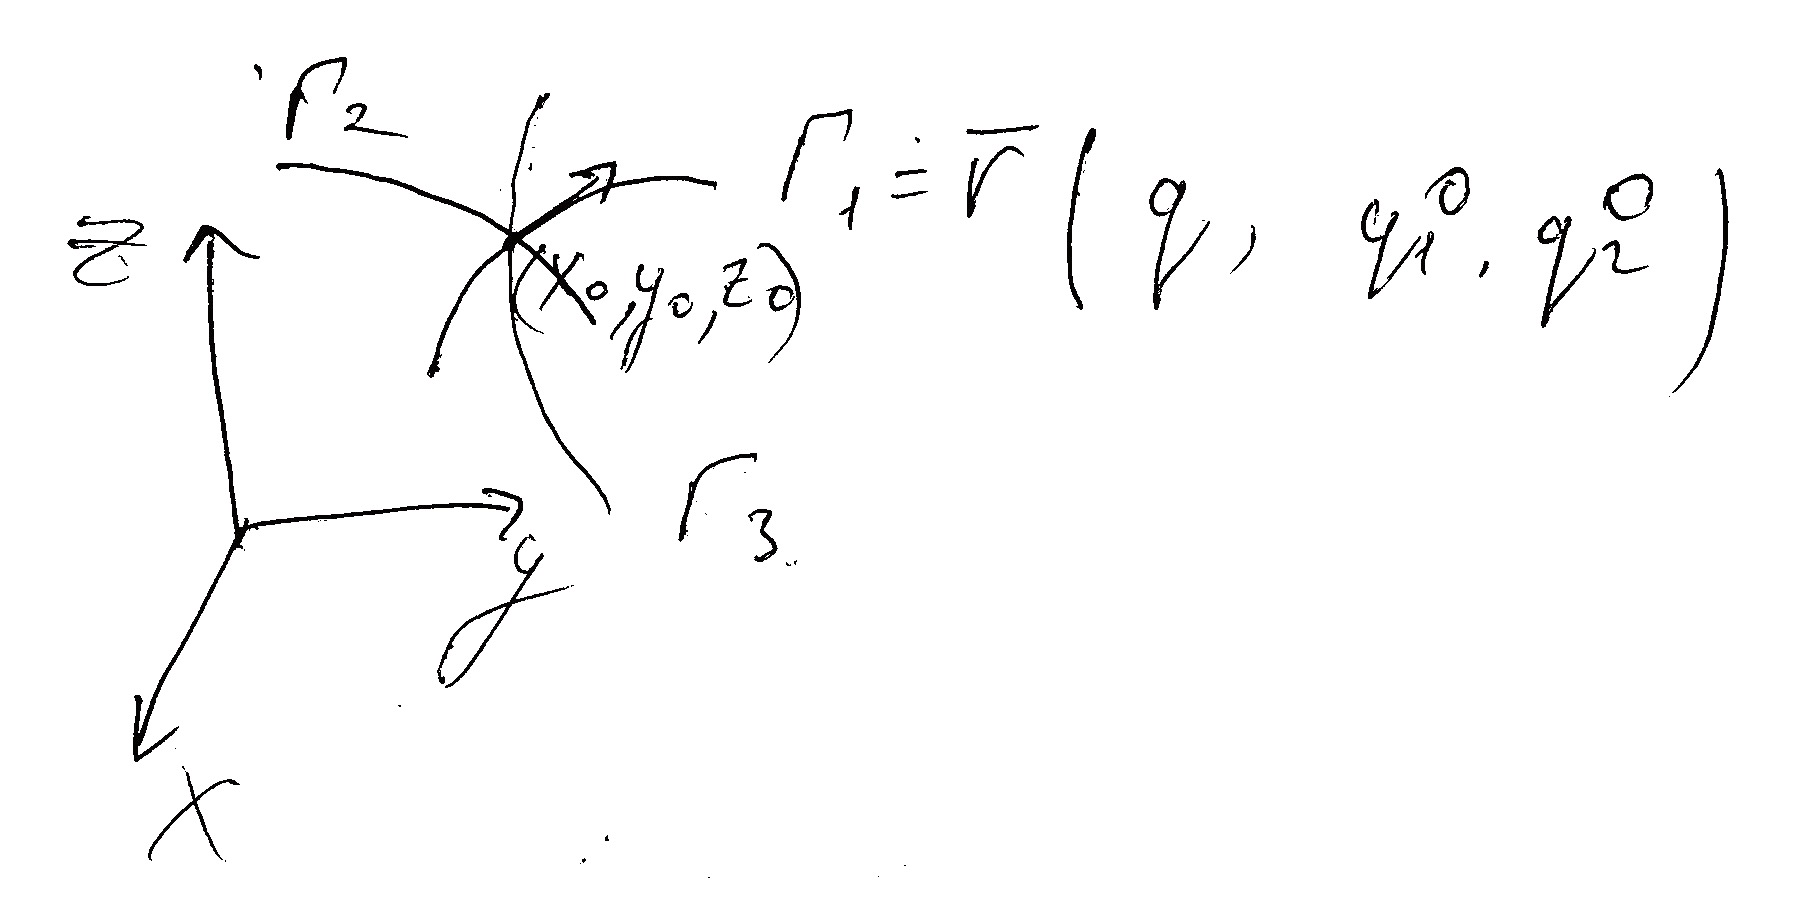
\includegraphics[width=0.5\textwidth]{КоординатныеЛинии.jpg}
    \caption{}
    \label{fig:myimage} % Sets a label for cross-referencing
\end{figure}
Появился касательный вектор к координатной линии $\Gamma_i$, орт локального базиса:
\[\bar e_i = \frac{\partial \bar r}{\partial q_i} / \left| \frac{\partial \bar r}{\partial q_i} \right|\]
\Def Коэффициент Ламе
\[H_i = \left| \frac{\partial \bar r}{\partial q_i} \right| \qquad \bar e_i = \frac{1}{H_i} \frac{\partial r}{\partial q_i}\]
Замечание: этот базис необязательно ортогональный
\\
Тогда скорость можно переписать как
\[\bar v = \sum_{i = 1}^3 \bar e_i H_i \dot q_i\]
\subsection{ОНЛБ}
Для ортонормированного локального базиса справедливо:
\[v = \sqrt{H_1^2 \dot q_1^2 + H_2^2 \dot q_2^2 + H_3^2 \dot q_3^2 }\]
\section{Ускорение}
\[
\bar v = \begin{pmatrix}v_1 \\ v_2 \\ v_3 \end{pmatrix} \qquad v_i = H_i \dot q_i
\]
В ОНЛБ:
\[
\begin{aligned}
w_i = (\bar w, \bar e_i) &= \left(\frac{d}{dt} \bar v, \frac{1}{H_i} \frac{\partial \bar r}{\partial q_i}\right) = \frac{1}{H_i} \left( \frac{d}{dt} \bar v, \frac{\partial \bar r}{\partial q_i}\right) \\
&= \left| \text{дифференцируем скалярное произведение} \left(\bar v, \frac{\partial \bar r}{\partial q_i}\right) \text{и вырыжаем результат} \right| \\
&= \frac{1}{H_i} \left( \frac{d}{dt} \left(\bar v, \frac{\partial \bar r}{\partial q_i}\right) - \left(\bar v, \frac{d}{dt} \frac{\partial \bar r}{\partial q_i} \right) \right) \\
&\begin{array}[t]{l@{\qquad}l} % [t]
\bar v = \frac{\partial \bar r}{\partial q_1} \dot q_1 + \frac{\partial \bar r}{\partial q_2} \dot q_2 + \frac{\partial \bar r}{\partial q_3} \dot q_3
 & \frac{d}{dt} \frac{\partial \bar r}{\partial q_i} = \frac{\partial \bar v}{\partial q_i} 
 \\
\frac{\partial \bar v}{\partial \dot q_i} = \frac{\partial \bar r}{\partial q_i} 
& \frac{\partial v^2}{\partial q_i} = \frac{\partial}{\partial q_i} (\bar v , \bar v) = 2 \left(\bar v , \frac{\partial \bar v}{\partial q_i}\right) \\
\end{array} 
\\
&= \frac{1}{H_i} \left(\frac{d}{dt} \left(\bar v , \frac{\partial \bar v}{\partial \dot q_i}\right)- \left(\bar v, \frac{\partial \bar v}{\partial q_i}\right)\right) \\
&= \frac{1}{H_i} \left(\frac{1}{2} \frac{d}{dt}\frac{\partial v^2}{\partial \dot q_i} -  \frac{1}{2} \frac{\partial v^2}{\partial q_i}\right) = \boxed{\frac{1}{H_i}\left(\frac{d}{dt} \frac{\partial  \frac{v^2}{2}}{\partial \dot q_i} - \frac{\partial \frac{v^2}{2}}{\partial q_i}\right)}
\end{aligned}
\]
\section{Твёрдое тело}
\Def (Абсолютное) твёрдое тело — Система материальных точек, расстояние между которыми остаётся неизменным во всё время движения
\subsection{Положение твёрдого тела с неподвижной точкой}
\begin{figure}[H]
    \centering
    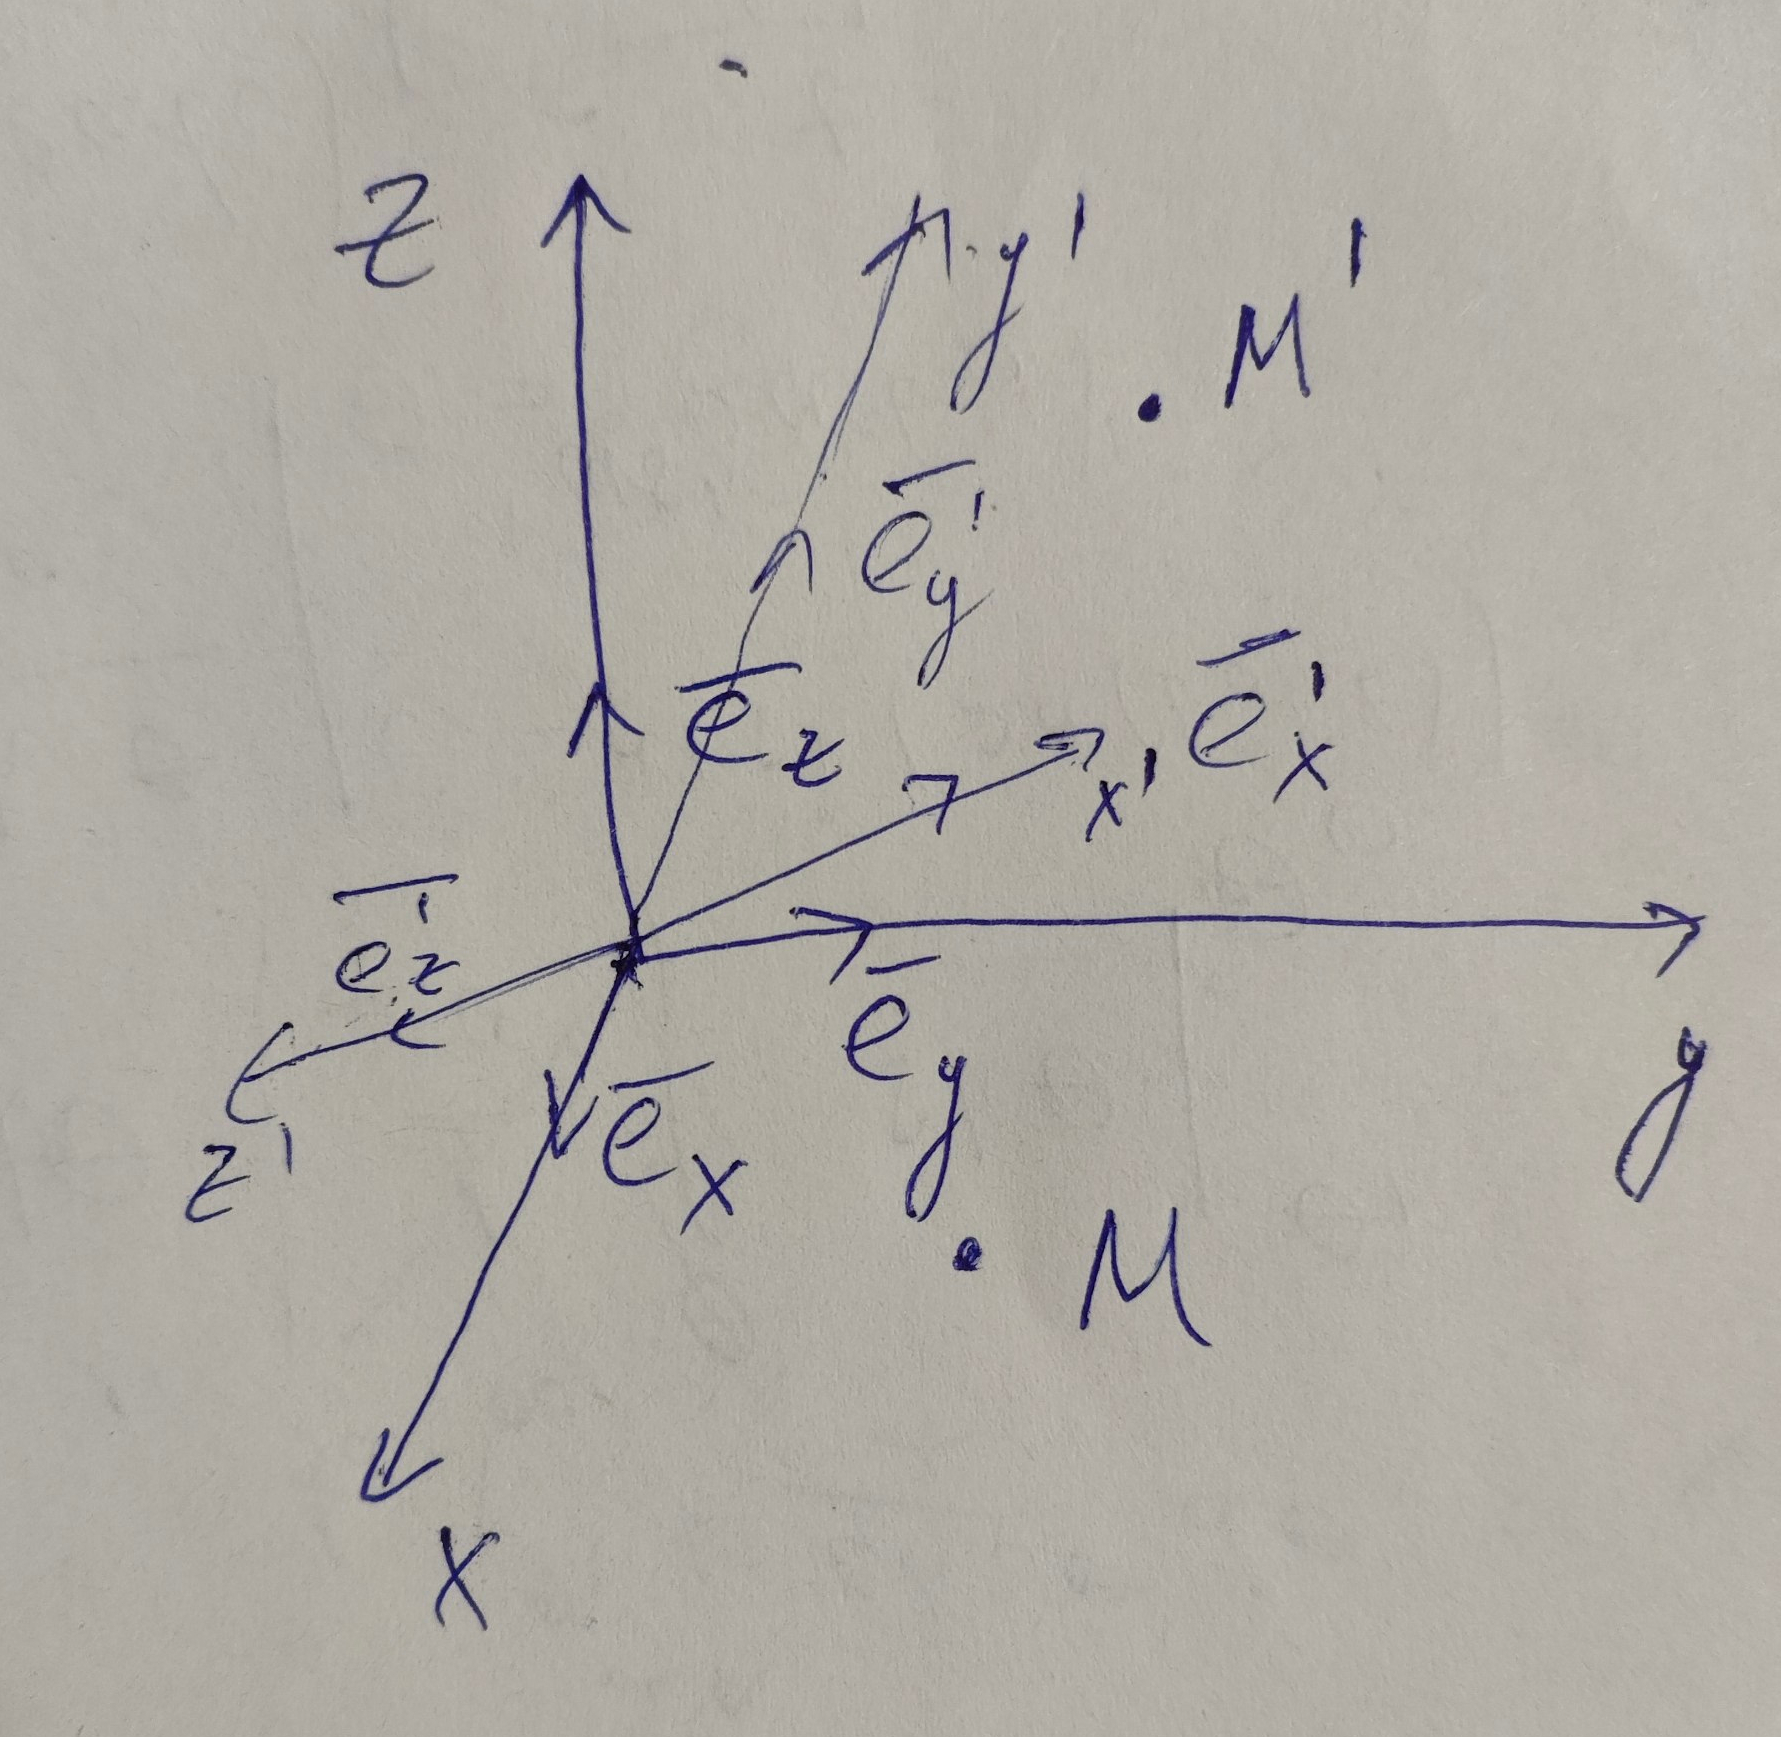
\includegraphics[width=0.5\textwidth]{ПоворотСК.jpg}
    \caption{}
    \label{fig:myimage} % Sets a label for cross-referencing
\end{figure}
\[M' \leftrightarrow M\]
\[\bar r = \bar f (\bar r')\]
\[Oxyz: \bar r = \begin{pmatrix}
    x \\ y \\ z
\end{pmatrix} = x \bar e_x + y \bar e_y + z \bar e_z = x' \bar e_{x'} + y' \bar e_{y'} + z' \bar e_{z'} = A \bar r'\]
$A$ — матрица перехода
\\
\Def $A$ — матрица направляющих косинусов, причём
\[\det A = 1\]
так как рассматриваем только повороты(без отражений)
\subsection{Свойства матрицы направляющих косинусов}
\begin{enumerate}
    \item 
    хорошее Доказательство, что $A^{-1} = A^T$ есть у Перескокова
    \item
    Элементы матрицы являются своими алгебраическими дополнениями
    \item 
    Собственные значения по модулю — единица
\end{enumerate}

\end{document}